\documentclass[10pt,conference,compsocconf]{IEEEtran}

% Language
%
\usepackage[english]{babel}
\usepackage[utf8]{inputenc}
\usepackage[T1]{fontenc}
\usepackage{hyphenat}
\usepackage{subfig}
\usepackage{float}
\usepackage{graphicx}
\usepackage{listings}

% Misc
%
\usepackage{xspace}
\usepackage{url}

% New commands
%
\newcommand\ConstructD{\textsf{Construct3D}\xspace}
\newcommand\MARIE{\textsf{MARIE}\xspace}
\newcommand\erlang{\textsf{Erlang}\xspace}
\newcommand\artoolkit{\textsf{ARToolKit}\xspace}
\newcommand\osgart{\textsf{OSGART}\xspace}
\newcommand\osg{\textsf{OpenSceneGraph}\xspace}
\newcommand{\cpp}{\textsf{C} \hspace*{-2.5mm} \raise 0.7mm \hbox {${\scriptscriptstyle ++}$}}
\newcommand\logo{\textsf{Logo}\xspace}

% Main
%
\begin{document}

\title{A Tangible Interface for Learning Recursion and Functional
  Programming}

\author{%
\IEEEauthorblockN{Juan Diego Tascón Vidarte}
\IEEEauthorblockA{Department of Advanced\\
Technology Fusion\\
Konkuk University\\
Seoul, Republic of Korea\\
\url{jtascon@konkuk.ac.kr}}
\and
\IEEEauthorblockN{Christian Rinderknecht}
\IEEEauthorblockA{Department of Internet\\
and Multimedia Engineering\\
Konkuk University\\
Seoul, Republic of Korea\\
\url{rinderkn@konkuk.ac.kr}}
\and
\IEEEauthorblockN{Jee-In Kim}
\IEEEauthorblockA{Department of Internet\\
and Multimedia Engineering\\
Konkuk University\\
Seoul, Republic of Korea\\
\url{jnkm@konkuk.ac.kr}}
\and
\IEEEauthorblockN{HyungSeok Kim}
\IEEEauthorblockA{Department of Internet\\
and Multimedia Engineering\\
Konkuk University\\
Seoul, Republic of Korea\\
\url{hyuskim@konkuk.ac.kr}}
}

\maketitle

%%-*-latex-*-

\begin{abstract}
Recursion is a powerful programming technique which is notoriously
difficult to master, especially in functional languages because they
prominently feature structural recursion as the main control\hyp{}flow
mechanism. We propose several hypotheses to understand the issue and
put some to the test by designing an open\hyp{}source interactive
interface based on a tangible block\hyp{}world with augmented reality
and software feedback. Stacks of blocks are used as an analogy for the
list data structure, which enables the simplest form of structural
recursion. After using this application, students are expected to
transfer their training to directly write recursive programs in
sequential \erlang, a purely functional language.
\end{abstract}


\begin{IEEEkeywords}
functional programming, tangible user interface, block world,
augmented reality, software feedback
\end{IEEEkeywords}

\IEEEpeerreviewmaketitle

%%-*-latex-*-

\section{Introduction}

The wide variety of software and hardware architectures in distributed
systems and telecommunications makes it valuable to use a common
high-level data notation in protocol specifications. To fulfill this
need, the ISO organization and the International Telecommunication
Union (ITU) defined the Abstract Syntax Notation One (\ASN) series of
standards. \ASN~\cite{Dubuisson:2000,X.680:2002,X.681:2002,X.682:2002,X.683:2002}
is a language for data types allowing the protocol designer to capture
numerous networking concepts, such as protocol data units, without
worrying about the possible environment and implementation
heterogeneity of the peers. The peers share a set of \ASN modules and
agree upon a set of \emph{encoding rules}, such
as~\cite{X.690:2002,X.691:2002}, which is a method for encoding values
produced at run-time by the communicating applications, into series of
bits. \ASN has been adopted for a wide range of applications, such as
network management, secure e-mail, mobile telephony, air traffic
control etc.
%, video conferencing over the internet, electronic commerce,
%digital certificates, radio paging, financial service systems etc.

\medskip

In the last few years, the press has reported several alleged
vulnerabilities of \ASN and the Basic Encoding Rules (BER) related to
network protocols like SNMP and, more recently, OpenSSL. Each time, an
accurate description of the problem has been finally published,
showing that the weakness lay in \emph{implementations} poorly written
and insufficiently tested. The real vulnerabilities were almost all
related to improper decoding of ill-formed BER encodings (or
\emph{codes}) causing buffer overflows, unspecified
(non-deterministic) behaviours, stack corruptions and, in the end, a
possible denial of service.

\medskip

From now on, it is important to understand and remember that \ASN and
the BER, intrinsically, have nothing to do with security or
cryptographic protocols. Both are used for modeling and handling the
data part of protocols, not the control. As a consequence, the
soundness property we aim at in this article must not be considered as
a security property about \emph{control} but as mere correctness of
composition of encoding and decoding with the BER of \emph{values}
specified by means of \ASN. For instance, there are no attackers, no
nonces etc. here. Nevertheless, the difficulty is not lesser.

\medskip

More precisely, in this work we want to prove that the design of the
BER themselves is flawless, whatever the network protocol is and
whatever the values to be transmitted are. To achieve this goal we
need the support of formal methods. We start by a formal modeling of
the BER which abstracts away low-level details but captures the design
principles. Then we define a soundness property representing the
security warranty we require and finally we prove that this property
holds for all values that can be specified with \ASN.


%%-*-latex-*-

\section{Methodology}

\noindent\textbf{System overview.} The application challenges the
student to solve a problem by interacting with stacks of blocks placed
on a table. A complete session is best understood as a series of
scenes, that is, snapshots of the board, which abstracts the execution
trace of an \erlang function on a given input, i.e., the initial
setting of the board. Markers are signs that are captured and
recognized by the system from the physical scene. They are
specifically designed to be easily understood by the \artoolkit (which
is a back\hyp{}end for \osgart) and are stuck on each block. They come
in three kinds: \textsl{Item}, \textsl{Stack} and \textsl{Switch}
(whose occultation by the hand triggers a snapshot). For each
recognized marker, a number, a variable, a picture may be superimposed
to the video feed and sent to a monitor. This 3D\hyp{}capable AR
feature is supported by another back\hyp{}end of \osgart called \osg.

\medskip

\noindent\textbf{Interactions.} The stack data structure can be
modified only by two simple operations: pop and push. These are the
minimum set of operations required to allow us to change the data in
any way we wish. However, in our system it is necessary to recognize
the block source and destination, that is, a stack, the table (it then
represents a value which is not a stack) or outside/inside the scene,
so the resulting set of operations is the following:
\begin{itemize}

  \item \textsl{Pop:} moving the top block from a stack onto the
    table;

  \item \textsl{Push}: moving a block from the table onto the top of a
    stack (dual of \textsl{Pop});

  \item \textsl{Pop-Push:} moving a top block from a stack on top of
    another stack (logical composition of \textsl{Pop} and
    \textsl{Push});

  \item \textsl{Discard:} moving a block or stack out of the scene,
    regardless of where it is located;

  \item \textsl{Create:} moving a block or a stack from outside the
    scene onto the table or the top of a stack (dual of
    \textsl{Discard}).
    
\end{itemize}
Changing a scene by any other means or by combining at once two or
more of these operations is considered invalid. These situations are
detected by the application which then stops the session with an error
message explaining what happened and prompts the student to restart
from scratch by placing the blocks back into a valid initial scene.

The system offers two execution modes: one called \emph{free},
allowing the student to freely, but validly, move blocks and another
one called \emph{supervised} in which each operation is checked to
conform to a possible solution, otherwise it is rejected and signalled
by a visual cue.

Adding new problems requires validating initial and final scenes and
dynamically creating \emph{positive scenarios}, that is, admissible
execution traces for different possible \erlang functions
corresponding to the problem. There are currently five problems
defined: stack reversal, joining two stacks, removing all the
occurrences of a given block in a stack, removing all consecutively
repeated blocks and sorting by insertion. The last two exercises are
more than structurally recursive because their assume some property on
the denotations of the blocks, equality and a total order,
respectively.

\bigskip

\noindent\textbf{A session.} Through the interface, blocks augmented
in yellow denote the base of stacks and light blue blocks represent
items belonging to a stack. The block with a camera icon projected
upon stands for the switch that, when hidden, triggers a scene
snapshot. A session ends with the system superimposing a
congratulation message if the student provides a correct and validly
obtained answer. In the case of an invalid action, the system displays
a message indicating the cause of the mistake, the blocks involved in
the invalid move will be augmented with red and the student will have
to restart the session from the beginning.

To illustrate how the interface works, we are going to step through a
sample session of the exercise consisting in joining two stacks, that
is, forming a new stack by moving all the items of one stack onto the
top of another, while retaining their original order. Textually, in
\erlang, this means that, given the stacks \texttt{P} and \texttt{Q},
with \texttt{P} denoting \texttt{[1,2]} (the top is \texttt{1} and the
bottom \texttt{2}) and \texttt{Q} denoting \texttt{[3,4]}, the joining
of \texttt{P} and \texttt{Q} is \texttt{[1,2,3,4]}. The user starts
the session by setting two stacks on the table, representing the input
arguments \texttt{P} (on the left) and \texttt{Q} (on the right) in
\erlang, i.e., \texttt{join(P,Q)} is the function call to
compute. Some random integers are superimposed on the blocks (they are
not random in the coming snapshots, so it is easier to follow the
transformations). This scene can be seen in
Figure~\ref{fig:head1}. 
\begin{figure}[!h]
\centering
\subfloat[\texttt{join([1,2],[3,4])}\label{fig:head1}]{
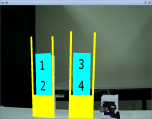
\includegraphics[scale=1.0]{step0.eps}
}
\quad
\subfloat[\texttt{join([],[1,2],[3,4])}\label{fig:body1}]{
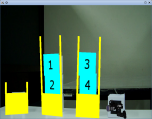
\includegraphics[scale=1.0]{step1.eps}
}
\caption{\texttt{\small join(P,Q) -> join([],P,Q)}
\label{fig:clause1}}
\end{figure}
The change of scene is denoted in \erlang by an arrow \texttt{->} at
the left of which is a pattern for the current scene and at the right
is the next scene in terms of the previous one. The final result
\texttt{[1,2,3,4]} is shown on the display and the user is prompted to
introduce from outside the scene an empty stack at the leftmost side
of the scene, which will be used as a temporary accumulator (operation
\textsl{Create}). This new scene is in Figure~\ref{fig:body1} and the
\erlang piece of code whose instanciation applies here is {\small
\begin{verbatim}
join(P,Q) -> join([],P,Q).
\end{verbatim}
}
\noindent 
where \texttt{[]} represents the empty stack. The user is now expected
to move top blocks from the middle stack (\texttt{P}) to the left
stack (operation \textsl{Pop\hyp{}Push}), as shown in
Figure~\ref{fig:clause2}.
\begin{figure}[!h]
\centering
\subfloat[\texttt{join([],[1,2],[3,4])}]{
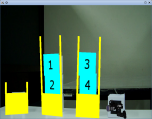
\includegraphics[scale=1.0]{step1.eps}
}
\quad
\subfloat[\texttt{join([1],[2],[3,4])}]{
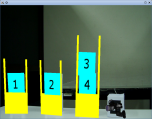
\includegraphics[scale=1.0]{step2.eps}
}
\caption{\texttt{\small join(A,[I|P],Q) -> join([I|A],P,Q)}
\label{fig:clause2}}
\end{figure}
This transformation is captured by the \erlang clause
{\small
\begin{verbatim}
join(A,[I|P],Q) -> join([I|A],P,Q);
\end{verbatim}
}
\noindent In \erlang, \texttt{[I|P]} is a pattern which matches any
non\hyp{}empty stack whose top block is named \texttt{I} and the
remaining stack \texttt{P}. After repeating this operation one more
time on our example, the scene is as shown in Figure~\ref{fig:head3}.
\begin{figure}[!h]
\centering
\subfloat[\texttt{join([2,1],[],[3,4])}\label{fig:head3}]{
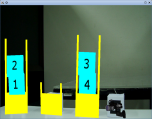
\includegraphics[scale=1.0]{step3.eps}
}
\quad
\subfloat[\texttt{join([1],[],[2,3,4])}\label{fig:body3}]{
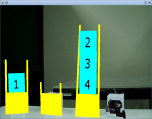
\includegraphics[scale=1.0]{step4.eps}
}
\caption{\texttt{\small join([I|A],[],Q) -> join(A,[],[I|Q])}
\label{fig:clause3}}
\end{figure}
It is matched by the pattern \texttt{join([I|A],[],Q)}, meaning ``left
stack with top block \texttt{I} and sub\hyp{}stack \texttt{A}, middle
stack empty and right stack \texttt{Q} unchanged.'' The next phase
consists in moving the blocks from the leftmost stack to the rightmost
(operation \textsl{Pop\hyp{}Push}). This is shown in
Figure~\ref{fig:clause3}, which corresponds to an instance of the
piece of source code 
{\small
\begin{verbatim}
join([I|A],[],Q) -> join(A,[],[I|Q]);
\end{verbatim}
}
\noindent After repeating this operation once more on our example, the
left stack becomes empty and the corresponding scene is seen in
Figure~\ref{fig:head4}. 
\begin{figure}[!h]
\centering
\subfloat[\texttt{join([],[],[1,2,3,4])}\label{fig:head4}]{
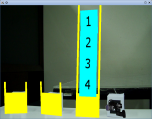
\includegraphics[scale=1.0]{step5.eps}
}
\quad
\subfloat[\texttt{[2,3,4]}\label{fig:body4}]{
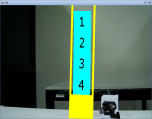
\includegraphics[scale=1.0]{step6.eps}
}
\caption{\texttt{\small join([],[],Q) -> Q}}
\label{fig:clause4}
\end{figure}
The \erlang pattern for it is \texttt{join([],[],Q)}. The result is
finally reached by keeping only the non\hyp{}empty stack on the scene
(operation \textsl{Discard} twice), as shown in
Figure~\ref{fig:clause4}. This is expressed by the clause
{\small
\begin{verbatim}
join([],[],Q) -> Q.
\end{verbatim}
} 
The student is not presented the \erlang at this stage, we wanted to
show the analogy between the AR scene and the textual program, which
the student in a later session will be asked to write directly. Here,
the complete \erlang program of this session was as follows (module
declarations omitted):
{\small
\begin{verbatim}
join(          P,Q) -> join(   [], P,    Q).
join(    A,[I|P],Q) -> join([I|A], P,    Q);
join([I|A],   [],Q) -> join(    A,[],[I|Q]);
join(   [],   [],Q) -> Q.
\end{verbatim}
}

\medskip

\noindent\textbf{Scope and limitations.} From the standpoint of
programming expressivity, the system is limited to functions based on
structural recursion on stacks and constant values. This is a
consequence of using a TUI, so adding new interactions would require
technologies that are not widely spread, for example gesture
recognition, motion tracking, voice recognition, etc. On the other
hand, with the current system, it just as easy to use rectangular
pieces of paper on a table instead of blocks, making it as portable as
the laptop with a webcam running it. The set of definable function is
also restricted to tail\hyp{}recursivity because representing the
control stack would require a special stack growing top\hyp{}down, so
the order of the instances of the control contexts is preserved. Since
the system is intended to be used by novices as a temporary tool to
understand simple cases of recursion, instead of as a general
programming environment, this is not an impediment.

\medskip

\noindent\textbf{Future experiments.} The first phase is made up of
three stages, which are repeated. In a first stage, the students will
be asked to build some stacks and randomly chosen integers will be
displayed on the blocks, one per block. The expected result will in
turn be shown on the screen. The student may select either the free or
supervised execution mode and try to reach the goal. After, two more
random examples for the same problem will be proposed. This stage
relies only on \emph{concrete examples}, as the one illustrated above
with \texttt{join}. It presents some similarities with the framework
of \emph{programming by example}, except that the goal is not to teach
the computer how to program but the other way round.

In the second stage, another random example for the same problem is
displayed but only the top of the stacks will be visible. This is
meant to induce in the learner the understanding that the exercise can
be solved without relying on global knowledge and that
\emph{information hiding} actually helps to focus the attention on the
smallest part of the data which is needed to make one more little step
towards the result. Each time a \textsl{Push\hyp{}Pop} operation is
performed, for instance, only the topmost blocks are consistently
shown.

After three runs like this, three other examples of the same problem
are offered, but instead of integers superimposed on the block
markers, \emph{variables} are. This last stage aims at giving rise to
\emph{abstraction} and prepares the transfer to textual programming.

When the last stage is over, another problem is submitted to the
student etc. until the interface hopefully becomes useless and the
direct programming of the \erlang functions corresponding to the
previous exercises is attempted. In the second phase, the professor
shows the analogy between, on the one hand, the stacks of blocks and
the valid operations learnt by means of the interface and, on the
other hand, the \erlang syntax for lists and the \erlang semantics. We
expect to measure a statistically significant transfer of training for
students who used the system in comparison with students who did not.


%%-*-latex-*-

\section{Conclusion\label{conclusion}}

In this paper we have presented a global test architecture for  
distributed services including the generation of test sequences for
service components. Our approach was validated by a case study: a
France Telecom \audio service.

The full service was described using the SDL language, and the running
of the Hit-or-Jump algorithm showed no deadlocks and produced the test
sequences for all the components of the studied service.

For sake of simplicity, we have selected a component of the \audio service
that is at the very heart of the service, the conference bridge, and
which coordinates the other components and illustrates clearly what
one imagines a \audio service is. The other components were generic
components that can be present in other kind of telecommunication
services, and for which we also generated the corresponding tests. We
have produced the tests for the bridge component in its context, and
we translated them in the TTCN and MSC formats.

We have also defined an architecture for the tester, which combines an
active part (based on a stimulation of the implementation) and a
passive one (based on the observation of the exchanges between the
CORBA objects). 

The results we got show that the use of formal methods considerably
eases the task of the service designers and developers, and that they
are usable for real services. Since the design phase to the
implementation and test phases, we used formal description techniques
(SDL, TTCN, MSC) and a formal test methodology. Moreover, we showed it
is possible to test the service components in the context of the
others (and not artificially in isolation). We think this is a notable
step towards the validation and the design of reusable
service-components.



\bibliographystyle{IEEEtran}
\bibliography{IEEEabrv,isuvr2010,tangible}

\end{document}
